

\chapter{Resultados} \label{chap:resultados}

\begin{figure}[H]  % <-- Este cambio es clave para que no se brinque
	\centering
	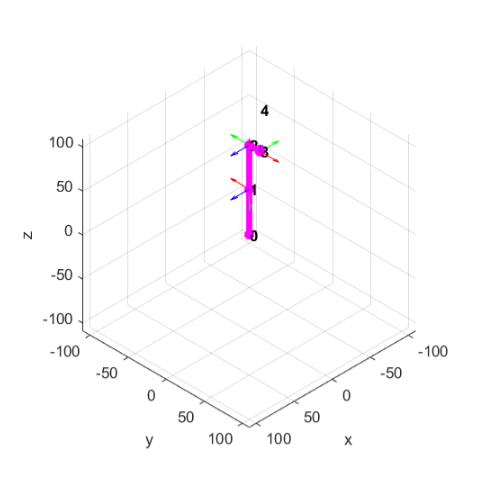
\includegraphics[width=0.7\linewidth]{img/grafica1directa}
	\caption{Representación tridimensional del robot con su sistema de coordenadas en cada eslabón. Se observa la posición y orientación del efector final en el espacio.}
	\label{fig:grafica1directa}
\end{figure}
La Figura 4.1 muestra la representación tridimensional del robot luego de aplicar la cinemática directa. Se visualizan los cuatro eslabones, así como los sistemas de coordenadas asociados a cada uno. Esta figura permite verificar visualmente que la configuración espacial del robot corresponde con los valores articulares definidos en la simulación.



\begin{figure}[H]
	\centering
	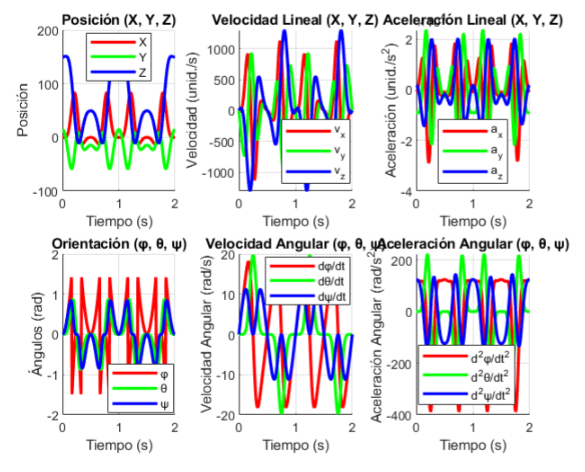
\includegraphics[width=0.9\linewidth]{img/imagen2directa}
	\caption{Resultados de la cinemática directa: posición, velocidad y aceleración lineal (superior), orientación, velocidad y aceleración angular (inferior) del efector final en función del tiempo.}
	\label{fig:imagen2directa}
\end{figure}
La Figura 4.2 presenta los resultados obtenidos a partir de la cinemática directa. En la primera fila se observan las componentes X, Y y Z de la posición, velocidad y aceleración lineal del efector final. En la segunda fila, se grafican los ángulos de Euler, así como sus derivadas primera y segunda (velocidad y aceleración angular). Estas gráficas permiten analizar el comportamiento dinámico del efector final a lo largo del tiempo.



\begin{figure}[H]
	\centering
	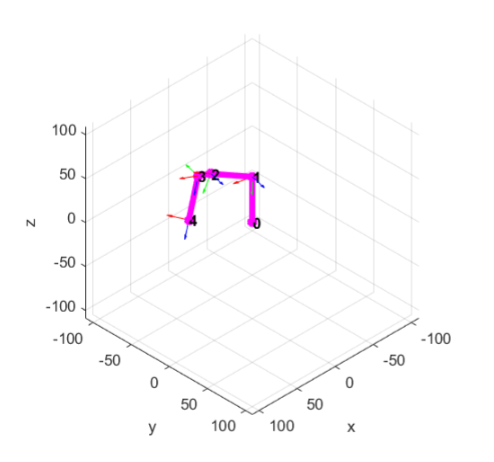
\includegraphics[width=0.7\linewidth]{img/inversa1}
	\caption{Representación 3D del robot en su entorno espacial durante la ejecución de la trayectoria.}
	\label{fig:inversa1}
\end{figure}
La Figura 4.3 muestra la animación del robot siguiendo una trayectoria predefinida en el espacio tridimensional. Las líneas representan los eslabones del robot, mientras que los ejes indican la orientación de cada articulación. Esta visualización fue generada durante la simulación de la cinemática inversa, donde el robot ajusta sus juntas para alcanzar puntos objetivos definidos por la trayectoria cartesiana.


\begin{figure} [H]
	\centering
	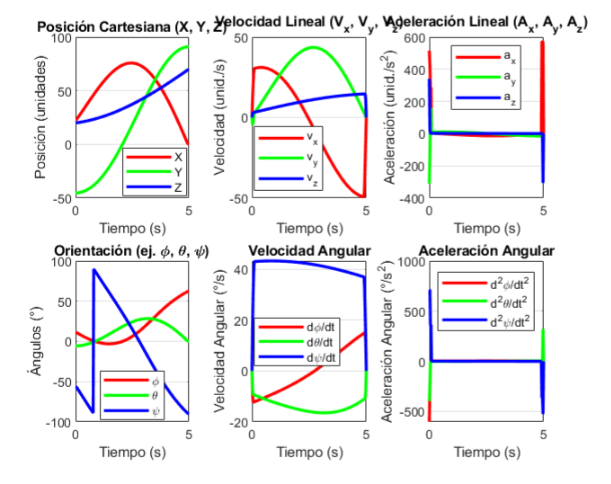
\includegraphics[width=0.9\linewidth]{img/inversa2}
	\caption{Comportamiento de la trayectoria cartesiana del efector final: posición, velocidad y aceleración lineal y angular.}
	\label{fig:inversa2}
\end{figure}
La Figura 4.4 muestra la evolución temporal de la posición (X, Y, Z), la velocidad y aceleración lineal del efector final, así como su orientación (ángulos de Euler), velocidad angular y aceleración angular. Estos resultados provienen de la cinemática directa aplicada a los ángulos articulares obtenidos mediante la cinemática inversa. Se puede observar que las curvas siguen un perfil suave, lo cual es crucial para garantizar un movimiento continuo y estable del robot.



\begin{figure} [H]
	\centering
	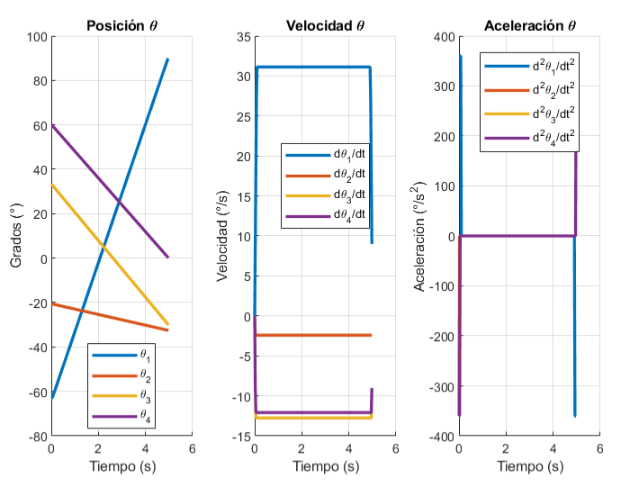
\includegraphics[width=0.9\linewidth]{img/inversa3}
	\caption{Trayectoria articular del robot: posición, velocidad y aceleración de las juntas.}
	\label{fig:inversa3}
\end{figure}
La Figura 4.5 representa el comportamiento de las variables articulares del robot a lo largo del tiempo. Se observa cómo cada articulación cambia su posición en grados, así como su velocidad y aceleración angular. Las trayectorias fueron generadas utilizando perfiles trapezoidales, lo que permite una transición suave entre los estados iniciales y finales, respetando los límites de velocidad y aceleración definidos para el robot.


















